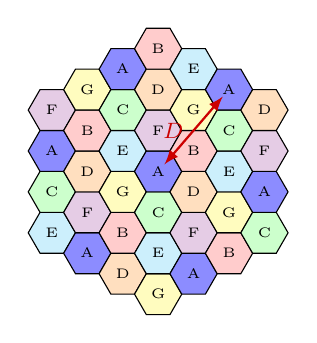
\begin{tikzpicture}[>=latex]
    \colorlet{cell0}{blue!45}
    \colorlet{cell1}{red!20}
    \colorlet{cell2}{green!20}
    \colorlet{cell3}{orange!25}
    \colorlet{cell4}{cyan!20}
    \colorlet{cell5}{violet!20}
    \colorlet{cell6}{yellow!25}
    \def\hexcell#1#2#3{\draw[fill=#3, shift={(#1,#2)}] (0:0.3) -- (60:0.3) -- (120:0.3) -- (180:0.3) -- (240:0.3) -- (300:0.3) -- cycle;}

    % Hexagonal grid, cells with the same letter share one channel set (N = 7)
    \foreach \q in {-3,...,3} {
        \foreach \v in {-3,...,3} {
            \pgfmathtruncatemacro{\dist}{max(abs(\q),abs(\v),abs(\q+\v))}
            \ifnum\dist<4
                \pgfmathtruncatemacro{\c}{mod(mod(\q+5*\v,7)+7,7)}
                \pgfmathsetmacro{\cx}{0.45*\q}
                \pgfmathsetmacro{\cy}{0.5196*(\v+0.5*\q)}
                \hexcell{\cx}{\cy}{cell\c}
                \node[font=\tiny] at (\cx,\cy) {\ifcase\c A\or B\or C\or D\or E\or F\or G\fi};
            \fi
        }
    }

    % Co-channel distance between two "A" cells: axial offset (2,1)
    \draw[<->, thick, red!80!black] (0.08,0.09) -- (0.82,0.95)
        node[midway, left, font=\footnotesize, text=red!80!black] {$D$};
\end{tikzpicture}
